\frame{
%\title{}
\begin{block}{A physical problem}
\begin{itemize}
\item  A spherical ball of radius $r$ is submerged to a depth $d$ in water. 
\item Assume that the ball is constructed from a variety of longleaf pine that has a density of $\rho = 0.638$ and that its radius measures $r = 10 cm$. 
\item How much of the ball will be submerged when it is placed in water?
\end{itemize}
\end{block}
\begin{figure}
\begin{center}
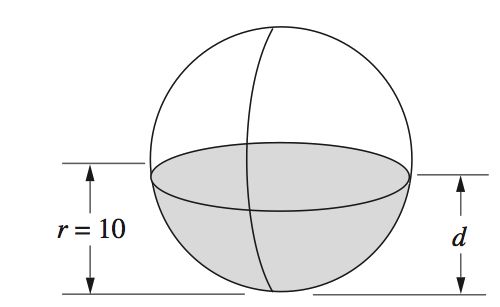
\includegraphics[width=45mm]{chap-1/fig_2-1.png}
%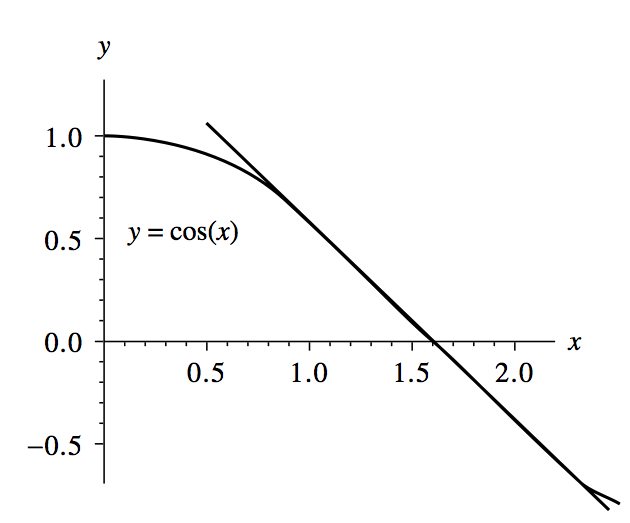
\includegraphics[width=45mm]{fig/ch-1/fig_1-1.png}
\caption{The portion of a sphere of radius $r$ that is to be submerged to a depth $d$}
\end{center}
\end{figure}
}

\frame{
%\begin{block}{}
\begin{itemize}
\item The mass $M_w$ of water displaced when a sphere is submerged to a depth $d$ is
\begin{equation*}
M_w = \int_0^d \pi (r^2 - (x-r)^2) dx = \frac{\pi d^2(3r-d)}{3}
\end{equation*}
\item the mass of the bell is 
\begin{equation*}
M_b = 4 \pi r^3 \rho \slash 3
\end{equation*}
\end{itemize}
%\end{block}
}

\frame{
\begin{columns}
\begin{column}{0.5\textwidth}
\begin{equation*}
\begin{array}{c}
M_w = M_b \\
\Downarrow \\
\frac{\pi(d^3 - 3d^2r + 4r^3 \rho)}{3} = 0 \\
\Downarrow \\
\frac{\pi(2552 - 30d^2 + d^3)}{3} = 0 \\
\Downarrow \\
y = 2552 -30d^2 + d^3
\end{array}
\end{equation*}
\end{column}
\begin{column}{0.5\textwidth}
\begin{figure}
\begin{center}
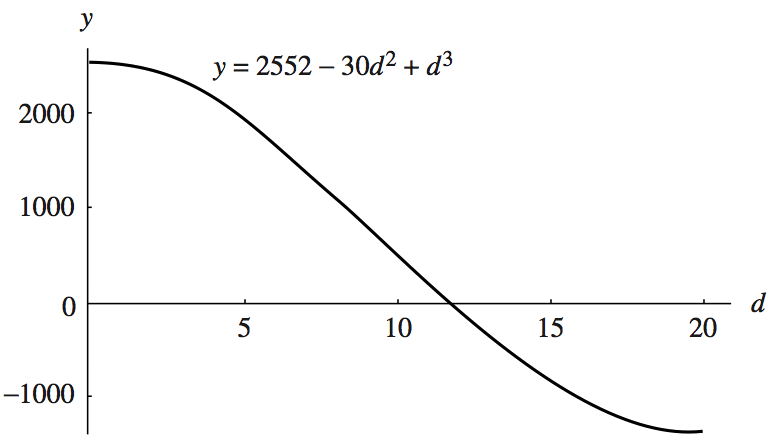
\includegraphics[width=45mm]{chap-1/fig_2-2.png}
%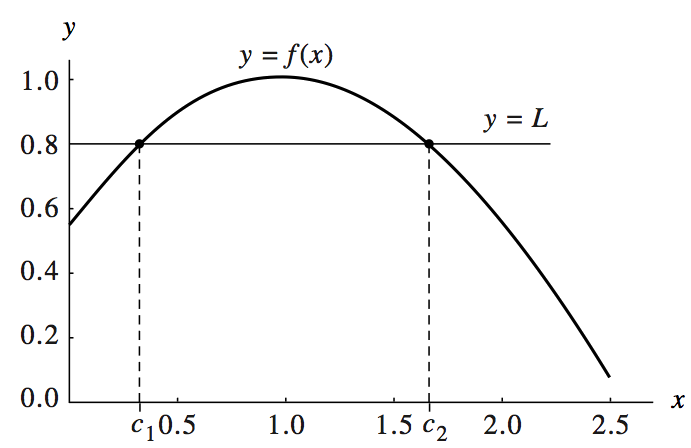
\includegraphics[width=55mm]{fig/ch-1/fig_1-2.png}
\caption{The cubic $y = 2552 - 30d^2 + d^3$}
\end{center}
\end{figure}
\end{column}
\end{columns}
\begin{center}
$\Downarrow $
\end{center}
\begin{block}{Solutions}
\begin{equation*}
\begin{array}{l l}
d_1 & = -8.17607212 \\
{\color{red} d_2} & {\color{red} = 11.86150151} \\
d_3 & = 26.31457061
\end{array}
\end{equation*}
\end{block}
}
